%%%%%%%%%%%%%%%%%%%%%%%%%%%%%%%%%%%%%%%%% 
% Landscape Poster
% LaTeX Template from Overleaf
% Version 1.0 (11/11/19)
% 
% 
% Further modified by:
% Chang Liao (changliao.climate@gmail.com)
% search "Chang comment" for help
% 
% 
% License:
% CC BY-NC-SA 3.0 (http://creativecommons.org/licenses/by-nc-sa/3.0/)
% 
%%%%%%%%%%%%%%%%%%%%%%%%%%%%%%%%%%%%%%%%% 
% ----------------------------------------------------------------------------------------
% PACKAGES AND OTHER DOCUMENT CONFIGURATIONS
% ----------------------------------------------------------------------------------------
\documentclass[final]{beamer}
% \usepackage[scale=1.24]{beamerposter}
\usepackage[orientation=landscape,size=a0,scale=1.4,debug]{beamerposter}% Use the beamerposter package for laying out the poster
\usetheme{confposter} % Use the confposter theme supplied with this template
\setbeamercolor{block title}{fg=ngreen,bg=white} % Colors of the block titles
\setbeamercolor{block body}{fg=black,bg=white} % Colors of the body of blocks
\setbeamercolor{block alerted title}{fg=white,bg=pnnl-copper} % Colors of the highlighted block titles
\setbeamercolor{block alerted body}{fg=black,bg=dblue!10} % Colors of the body of highlighted blocks
% Many more colors are available for use in beamerthemeconfposter.sty
% -----------------------------------------------------------
% Define the column widths and overall poster size
% To set effective sepwid, onecolwid and twocolwid values, first choose how many columns you want and how much separation you want between columns
% In this template, the separation width chosen is 0.024 of the paper width and a 4-column layout
% onecolwid should therefore be (1-(# of columns+1)*sepwid)/# of columns e.g. (1-(4+1)*0.024)/4 = 0.22
% Set twocolwid to be (2*onecolwid)+sepwid = 0.464
% Set threecolwid to be (3*onecolwid)+2*sepwid = 0.708
%Chang comment: you can set up as many columns as you like, but you should do the math first here
\newlength{\sepwid}
\newlength{\onecolwid}
\newlength{\twocolwid}
\newlength{\threecolwid}
\newlength{\sidewid}
\setlength{\paperwidth}{60in} % A0 width: 46.8in
\setlength{\paperheight}{42in} % A0 height: 33.1in
\setlength{\sepwid}{0.01\paperwidth} % Separation width (white space) between columns
\setlength{\onecolwid}{0.32\paperwidth} % Width of one column
\setlength{\twocolwid}{0.46\paperwidth} % Width of two columns
\setlength{\threecolwid}{0.65\paperwidth} % Width of three columns
\setlength{\topmargin}{-1.0in} % Reduce the top margin size
\setlength{\sidewid}{0.1\paperwidth} % side background 

% -----------------------------------------------------------
\usepackage{graphicx} % Required for including images
\usepackage{pdfpages}
\usepackage[export]{adjustbox}
\usepackage{booktabs} % Top and bottom rules for tables
% Chang comment
% \usepackage{mathptmx}% http://ctan.org/pkg/mathptmx
% \usepackage[format=plain,font=footnotesize, captionlabelfont = plain]{caption}
\setbeamerfont{caption}{size=\footnotesize}
\setbeamerfont{caption name}{size=\footnotesize,series=\bfseries}
\renewcommand{\familydefault}{\rmdefault}
\usepackage{subcaption}
\setbeamertemplate{caption}[numbered]
\setbeamertemplate{headline}{
  \leavevmode
  \begin{columns}
    \begin{column}{ 1.1 \linewidth}      
      % \raggedright
      \vskip0.3in
      %\vspace{0.5in}
      \usebeamercolor{title in headline}{\color{black}\Huge{\textbf{\inserttitle}}\\[0.4ex]}      
      \usebeamercolor{author in headline}{\color{black}\Large{\insertauthor}\\[0.4ex]}
      \usebeamercolor{institute in headline}{\color{black}\large{\insertinstitute}\\[0.4ex]}
      %\vskip0.5in
    \end{column}    
  \end{columns}  
  % \hspace{0.5in}\begin{beamercolorbox}[wd=47in,colsep=0.15cm]{cboxb}\end{beamercolorbox}
  %\vspace{0.5in}
}
%Chang comment: this is where you can modify the background image
\setbeamertemplate{background}{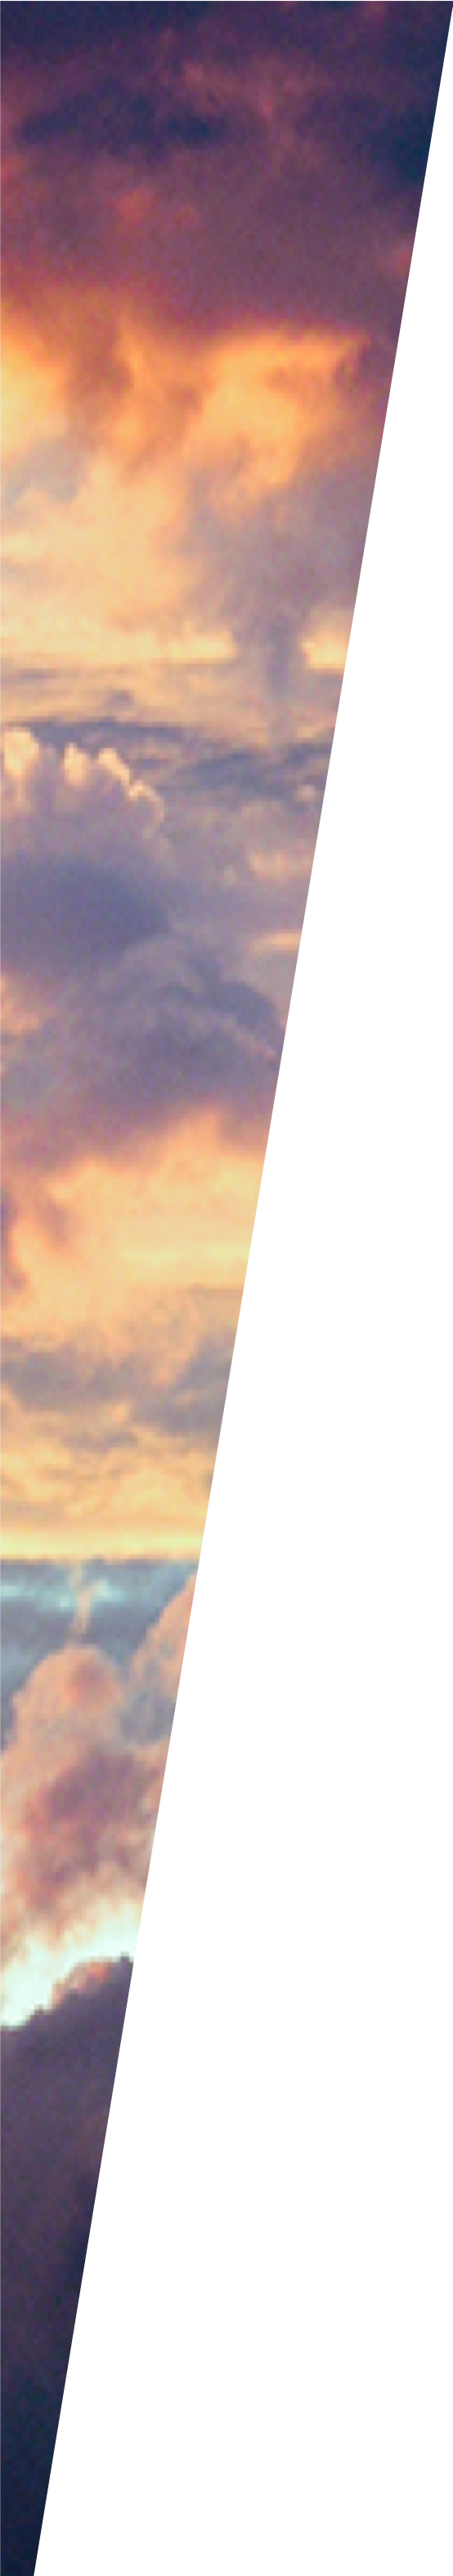
\includegraphics[height=\paperheight, keepaspectratio]{figure/background2019.png}}
% ----------------------------------------------------------------------------------------
% TITLE SECTION
% ----------------------------------------------------------------------------------------
%Chang comment: this is one of the projects we finished.
\title{ \huge{  \hspace{4.5in} Watershed Delineation On A Hexagonal Mesh Grid}}
\author{ \Large{ \hspace{6in} Chang Liao, Teklu Tesfa, Zhuoran Duan, and Ruby Leung } }
\institute[ETH]{
  \large{ \hspace{6in} Pacific Northwest National Laboratory }}
\date{\today}


% ----------------------------------------------------------------------------------------
\begin{document}
\addtobeamertemplate{block begin}{}{\vspace*{0.2ex}} % White space under blocks
\addtobeamertemplate{block end}{}{\vspace*{0.5ex}} % White space under blocks
\addtobeamertemplate{block alerted end}{}{\vspace*{1ex}} % White space under highlighted (alert) blocks
\setlength{\belowcaptionskip}{1ex} % White space under figures
\setlength\belowdisplayshortskip{1ex} % White space under equations
\begin{frame}[t] % The whole poster is enclosed in one beamer frame
  \vspace{-3in}
  \begin{columns}[t] % The whole poster consists of three major columns, the second of which is split into two columns twice - the [t] option aligns each column's content to the top
    \begin{column}{\sidewid}
    \end{column} % Empty spacer column
    \begin{column}{\sepwid}
    \end{column} % Empty spacer column
    \begin{column}{\onecolwid} % The first column
      \vspace{4.0in} % The first column within column 2     
      % ----------------------------------------------------------------------------------------
      % INTRODUCTION
      % ----------------------------------------------------------------------------------------
      \begin{block}{Background}
        % footnotesize normalsize
        Spatial discretization is the cornerstone of all spatially-distributed numerical simulations including watershed hydrology. Traditional square grid spatial discretization inevitably suffers from several drawbacks.   
        First, square grid spatial discretization (SGSD) cannot uniformly represent adjacency. The diagonal neighbors are further than the direct ones (Figure \ref{fig:d4d8}). However, these differences are not treated consistently under different circumstances. Second, SGSD will create isolated ``island'' due to the differences in D4 and D8 definitions (Figure \ref{fig:island}).
        Third, SGSD cannot effectively represent a spherical topology, which will bring significant spatial distortions regardless of Geographic Coordinate Systems (GCS) or Projected Coordinate Systems (PCS) used.

        In contrast, HGSD can resolve these drawbacks effortlessly (Figure \ref{fig:d6}). For example, it can provide global coverage using the Icosahedron Snyder Equal Area (ISEA) mesh grid.
        \begin{figure}[H]
          \centering
          \begin{subfigure}[t]{0.3\textwidth}
            \centering
            
\includegraphics[width=\linewidth]{figure/placeholder.jpg}
            \caption{}
            \label{fig:d4d8}
          \end{subfigure}
          \begin{subfigure}[t]{0.3\textwidth}
            \centering
            
\includegraphics[width=\linewidth]{figure/placeholder.jpg}
            \caption{}
            \label{fig:island}
          \end{subfigure}
          \begin{subfigure}[t]{0.3\textwidth}
            \centering
            
\includegraphics[width=\linewidth]{figure/placeholder.jpg}
            \caption{}
            \label{fig:d6}
          \end{subfigure}
          \caption{Illustration of traditional D4 and D8 neighbor definitions, the ``island'' effect, and the D6 neighbor definition. (a) green and red arrows represent direct and diagonal neighbors, respectively. (b) grid 1 is an isolated island but it's a D8 neighbor of grid 2. (c) is D6 neighbor definition.}
          \label{fig:d4d8_island_d6}
        \end{figure}
      \end{block}
      \begin{block}{Method}
        Following the algorithms which were used in traditional watershed delineation method, we developed a list of algorithms for the HGSD method: DEM depression filling, flow direction, flow accumulation, stream definition, etc.
        We also evaluated the model performance again the traditional method and the NHD datasets (Figure \ref{fig:cbc}).
      \end{block}
      \begin{alertblock}{Conclusion}
        Because of the consistent connectivity, nearly all spatial distributions of watershed characteristics (e.g., flow direction and stream networks) are closer to the reality at various resolutions.
        Our analysis implies that spatially-distributed hydrological simulation which relies on connectivity/routing will be improved if we use the HGSD method.
      \end{alertblock}

      \setbeamercolor{block alerted title}{fg=white,bg=pnnl-silver} % Change the alert block title colors
      \setbeamercolor{block alerted body}{fg=black,bg=white} % Change the alert block body colors
      \begin{alertblock}{Acknowledgement}
        The research described in this poster was conducted under the Laboratory Directed Research and Development (LDRD) Program at Pacific Northwest National Laboratory (PNNL). A portion of this research was performed using PNNL Research Computing at Pacific Northwest National Laboratory.
      \end{alertblock}
      % ----------------------------------------------------------------------------------------
    \end{column} % End of the first column
    % \begin{column}{\sepwid}
    % \end{column} % Empty spacer column
    \begin{column}{\threecolwid}
      \vspace{10in}
      % ----------------------------------------------------------------------------------------
      % MATERIALS
      % -----------------------------------------------------------------------------------

      \begin{minipage}[b][0.3\textheight][c]{0.4\textwidth}
        \begin{figure}[ht]
          \begin{subfigure}[t]{\textwidth}
            \centering
            
\includegraphics[width=\linewidth]{figure/placeholder.jpg}
            \caption{Grid A.}
          \end{subfigure}
          \begin{subfigure}[t]{\textwidth}
            \centering
            
\includegraphics[width=\linewidth]{figure/placeholder.jpg}
            \caption{Grid B.}
          \end{subfigure}
        \end{figure}
          \end{minipage}
        \begin{minipage}[b][0.3\textheight][c]{0.4\textwidth}
          \begin{figure}
            
\includegraphics[width=\linewidth]{figure/placeholder.jpg}
            \caption{Calibrated soil anisotropy of hydraulic conductivity.}
            \label{fig:clm_structure}
          \end{figure}
        \end{minipage}

      \begin{figure}
        
\includegraphics[width = 0.72\textwidth]{figure/placeholder.jpg}
        \caption{Spatial distributions of simulated flow direction and stream networks in Columbia River Basin.}
        \label{fig:cbc}
      \end{figure}
    \end{column} % End of column 2.1    
  \end{columns} % End of all the columns in the poster
  \vspace{0in}
  \begin{columns}[t]   
    \begin{column}{\sepwid}
    \end{column} % Empty spacer column
    \begin{column}{\sepwid}
    \end{column} % Empty spacer column
    \begin{column}{0.9\paperwidth}      
      
\includegraphics[width=\textwidth,center]{figure/bottom_logo.png}     
    \end{column}   
    \begin{column}{\sepwid}
    \end{column} % Empty spacer column
  \end{columns}
\end{frame} % End of the enclosing frame
\end{document}
% unused text

